% !TEX TS-program = pdflatex
%% !TEX encoding = UTF-8 Unicode
% !TEX spellcheck = en_US

% This is a simple template for a LaTeX document using the "article" class.
% See "book", "report", "letter" for other types of document.

\documentclass[11pt]{paper} % use larger type; default would be 10pt

\usepackage{lineno}

\usepackage{setspace}
%\doublespacing

%%% Examples of Article customizations
% These packages are optional, depending whether you want the features they provide.
% See the LaTeX Companion or other references for full information.

%%% PAGE DIMENSIONS
%\usepackage{geometry} % to change the page dimensions
%\geometry{a4paper} % or letterpaper (US) or a5paper or....
% \geometry{margin=2in} % for example, change the margins to 2 inches all round
% \geometry{landscape} % set up the page for landscape
%   read geometry.pdf for detailed page layout information
\usepackage{mathtools}
\usepackage{graphicx} % support the \includegraphics command and options
\usepackage{caption}
\usepackage{subcaption}
\usepackage{wrapfig}
\usepackage[leftcaption]{sidecap}

\graphicspath{{./}{./fig/}}

\usepackage[style=numeric-comp, sorting=none, url=false, isbn=false]{biblatex}
\addbibresource{binding-pocket.bib}

% \usepackage[parfill]{parskip} % Activate to begin paragraphs with an empty line rather than an indent

%%% PACKAGES
%\usepackage{booktabs} % for much better looking tables
%\usepackage{array} % for better arrays (eg matrices) in maths
%\usepackage{paralist} % very flexible & customisable lists (eg. enumerate/itemize, etc.)
%\usepackage{verbatim} % adds environment for commenting out blocks of text & for better verbatim
%\usepackage{subfig} % make it possible to include more than one captioned figure/table in a single float
% These packages are all incorporated in the memoir class to one degree or another...

%%% HEADERS & FOOTERS
%\usepackage{fancyhdr} % This should be set AFTER setting up the page geometry
%\pagestyle{fancy} % options: empty , plain , fancy
%\renewcommand{\headrulewidth}{0pt} % customise the layout...
%\lhead{}\chead{}\rhead{}
%\lfoot{}\cfoot{\thepage}\rfoot{}

%%% SECTION TITLE APPEARANCE
%\usepackage{sectsty}
%\allsectionsfont{\sffamily\mdseries\upshape} % (See the fntguide.pdf for font help)
% (This matches ConTeXt defaults)

%%% ToC (table of contents) APPEARANCE
%\usepackage[nottoc,notlof,notlot]{tocbibind} % Put the bibliography in the ToC
%\usepackage[titles,subfigure]{tocloft} % Alter the style of the Table of Contents
%\renewcommand{\cftsecfont}{\rmfamily\mdseries\upshape}
%\renewcommand{\cftsecpagefont}{\rmfamily\mdseries\upshape} % No bold!

%%% END Article customizations

%%% The "real" document content comes below...

\title{Olfactory receptors of Drosophila are sensitive to molecular volume of odorants}
\author{Majid Saberi \and Hamed Seyed-allaei\thanks{hamed@ipm.ir}}
\institution{School of Cognitive Science, \\ Institute for Research in Fundamental Sciences (IPM), \\Tehran, Iran}
%Olfactory System; Olfactory Receptor; Chemical Range; G Protein-Coupled Receptors; Odor-Structure Relation;
%Majid Saberi <majidsaberi048@gmail.com>
%leslie.vosshall@rockefeller.edu
%giovanni.galizia@uni-konstanz.de
%m.schmuker@biomachinelearning.net Michael Schmuker

%\date{} % Activate to display a given date or no date (if empty),
         % otherwise the current date is printed 

\newcommand{\numberofreceptors}{ 28 }
\newcommand{\bonferroni}{ 11 }
\newcommand{\fdr}{ 26 }
\newcommand{\nocorrection}{ 2 }

\begin{document}


%\linenumbers

\maketitle

\begin{abstract} 
Which properties of a molecule define its odor? This is a basic question of olfaction, 
yet to be answered. Human olfactory system has a repertoire of about 350 olfactory receptors. 
Molecules bind to them with different affinities and activate them with different efficacies, 
resulting in a combinatorial code that identifies odorants. 
We hypothesized that the binding affinity between a pair of odorant-receptor is affected by their relative sizes. 
The affinity can reaches its maximum if molecular volume of an odorant matches volume of a receptor's binding-pocket 
and it reach zero if the sizes are too different, 
obscuring the effect of other molecular properties. 
We formulated this hypothesis mathematically and verified it on Data of Drosophila, 
and predicted the volume and the structural flexibility of each receptor's binding-site, 
which are significantly different among receptors. 
This provides a reason for differences in smell among similar molecules of different sizes. 
\end{abstract}



%\section*{Significance Statement}
%We perceive wavelength of light as its colors and frequency of sound as its pitch. But we don’t know yet what properties of molecules are perceived as smell. In this work, for the first time, we showed that molecular volume of an odorant is an important factor in the fruit fly. It affects two dimensions of smell: its intensity (weak or strong) and its quality (sweet, floral, fruity or etc). The molecular volume could describe the difference in the smell of methanol and butanol. Methanol smells pungent while butanol smells winy with a tad of banana like aroma.

\section*{Introduction}

%%%%%
I applied some combinations of test wells as baseline and see results of significancy of volume sensitivity in odorant receptors.
  
test well = 36 , data = data1 \&\ data2 , dens = 0 , ORs = 512:

sig= 74, fdr= 13, bon= 5.

test well = (36,48,60) , data = data1 , dens = 0 , ORs = 442:

sig= 124, fdr= 49, bon= 19.

test well = (72,84,96) , data = data1 , dens = 10 , ORs = 442:

sig= 71, fdr= 1, bon= 1.

test well = (12,24,36,48) , data = data2 , dens = 0 , ORs = 72:

sig= 2, fdr= 0, bon= 0.

test well = (60,72,84,96) , data = data2 , dens = 1 , ORs = 72:

sig= 0, fdr= 0, bon= 0.

test well = (36,48,60)(12,24,36,48) , data = data1 \&\ data2 , dens = 0 , ORs = 512:

sig= 123, fdr= 42, bon= 19.



\begin{figure}
	\centering
%	\begin{subfigure}[b]{\textwidth}
		\includegraphics[width=1 \textwidth]{vol-res-human-fdr}
		%\caption{}
		\label{fig:vol-res:all}		
%	\end{subfigure}
%	\begin{subfigure}[b]{0.75 \textwidth}
%		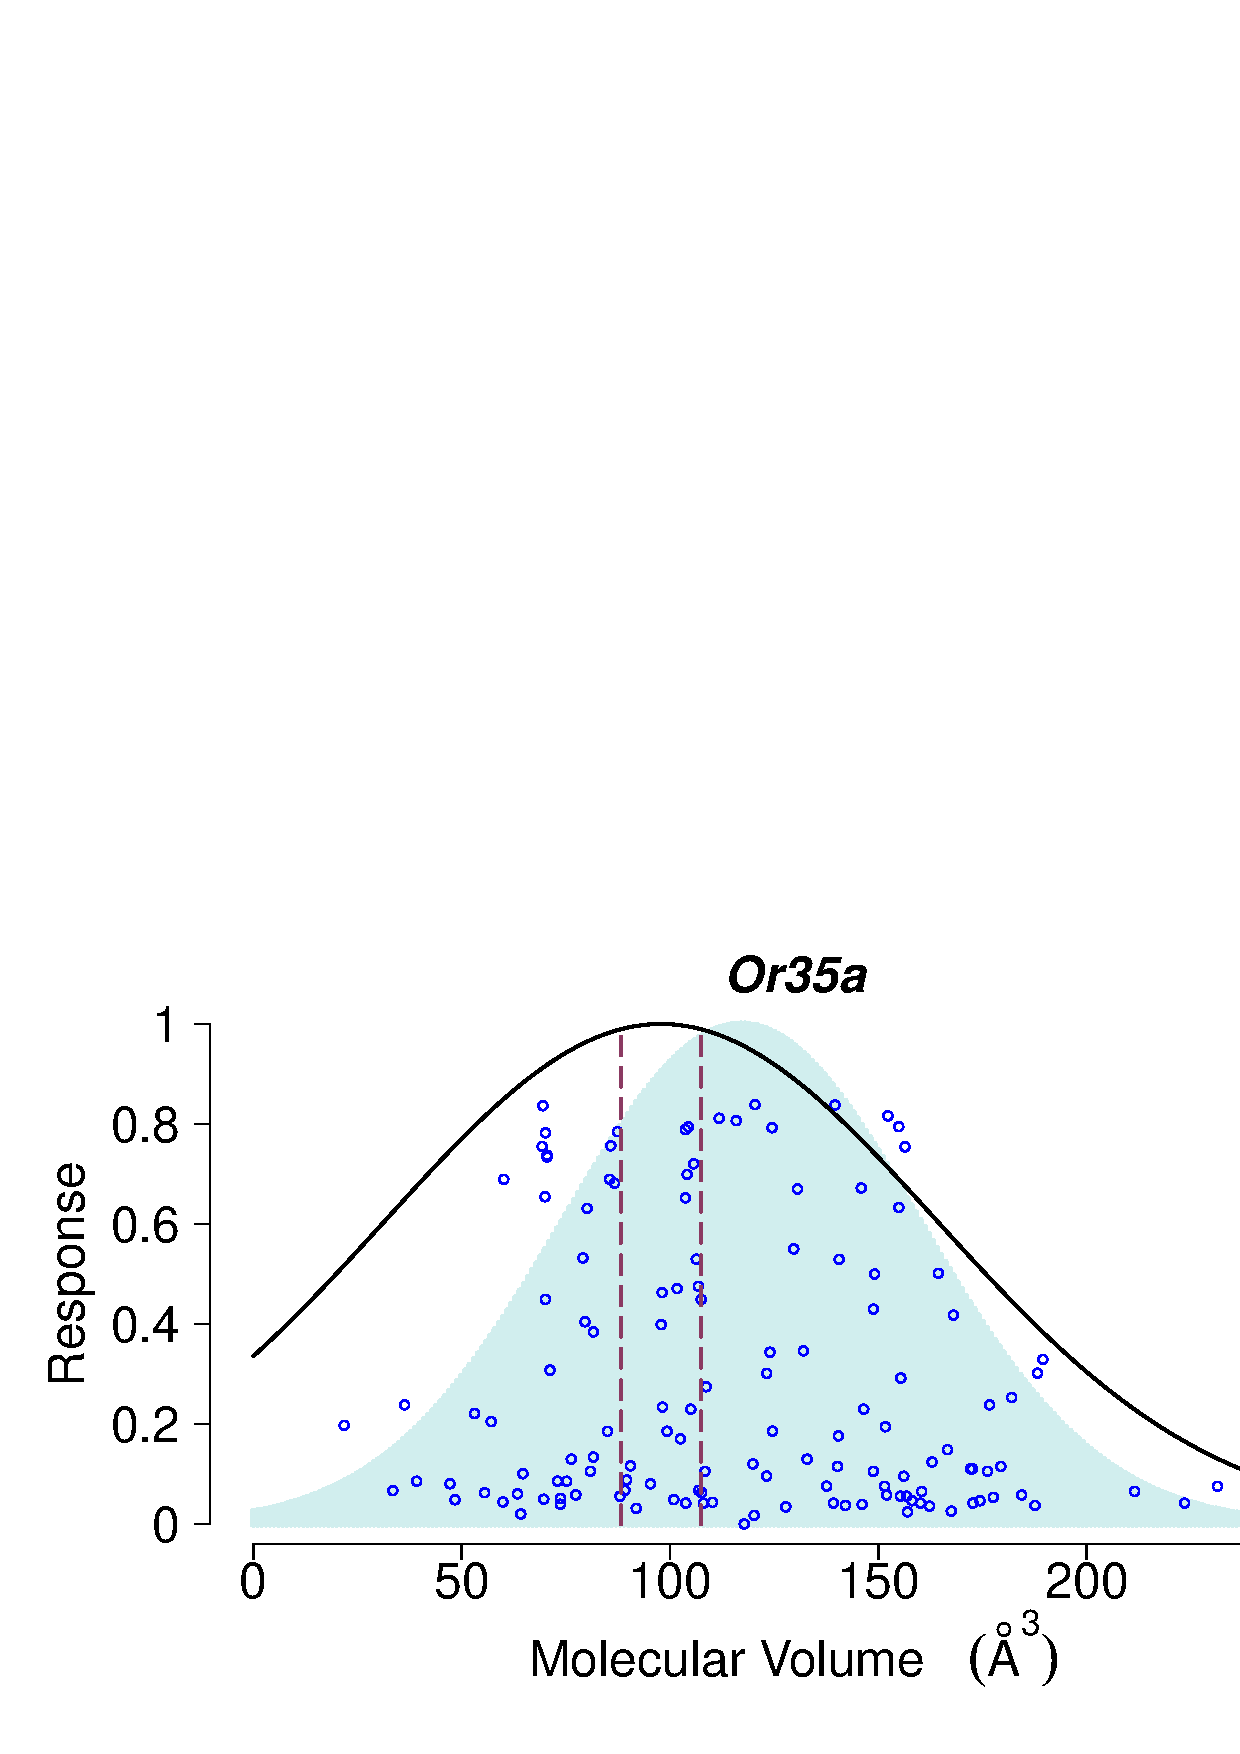
\includegraphics[width= \textwidth]{fig/vol-res-Or35a}
%		\caption{}	
%		\label{fig:vol-res:one}	
%	\end{subfigure}
	\caption{Response of olfactory receptors  versus molecular volume of odorants (circles),  
			the fitted functions $f_n(v)$ from Eq.~\ref{eqn:factors} (solid lines), 
			and the error bars of the mean of $f_n(v)$ (red vertical lines), 
			for \numberofreceptors receptors that their response showed significant FDR correction (p-value $<0.05$) dependence to molecular volume. 
			Among them, \fdr are significant according to FDR correction (receptor names in bold) and 
			\bonferroni are significant considering Bonferroni correction (receptor names in italic).
		}
	\label{fig:vol-res-human}
\end{figure}


\begin{figure}
%	\begin{subfigure}[b]{\textwidth}
		\centering
		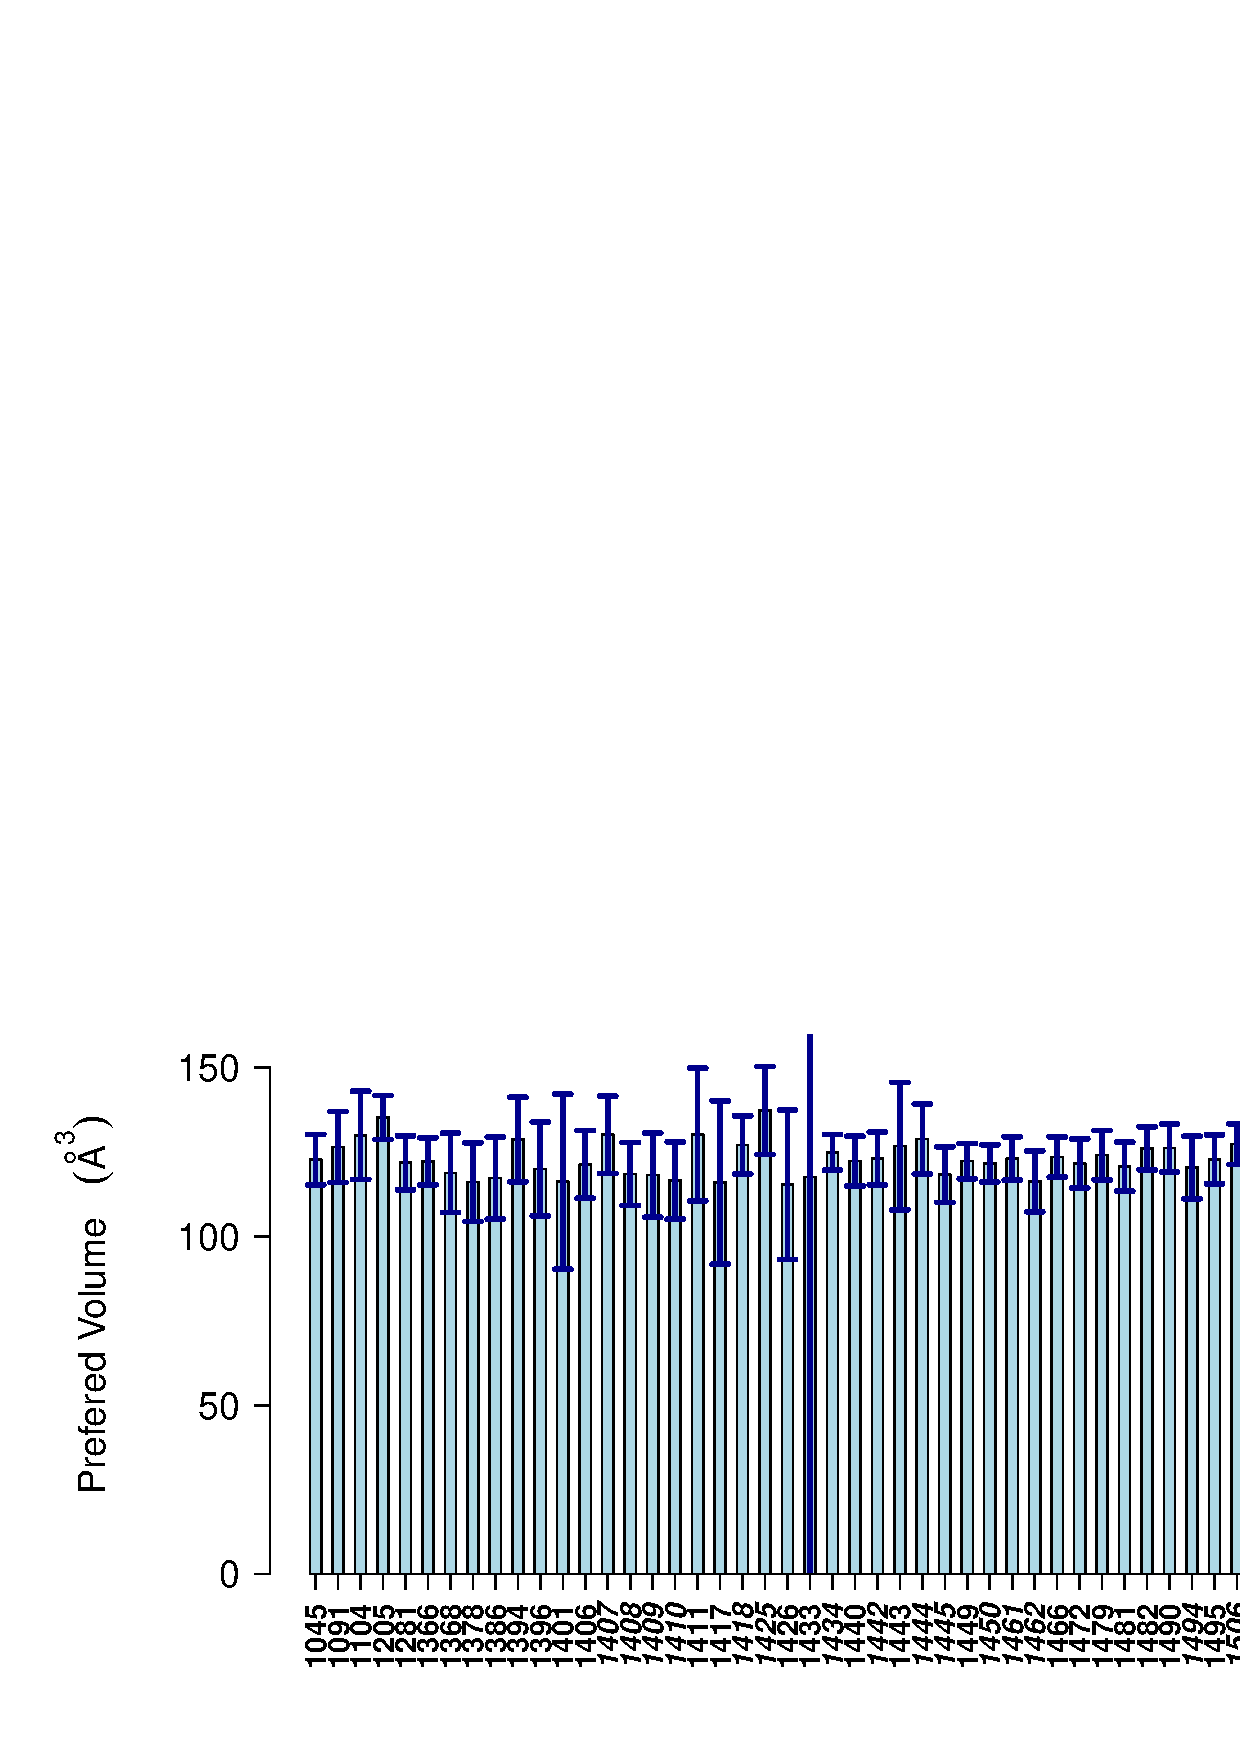
\includegraphics[width=  1 \textwidth]{mean-vol}
		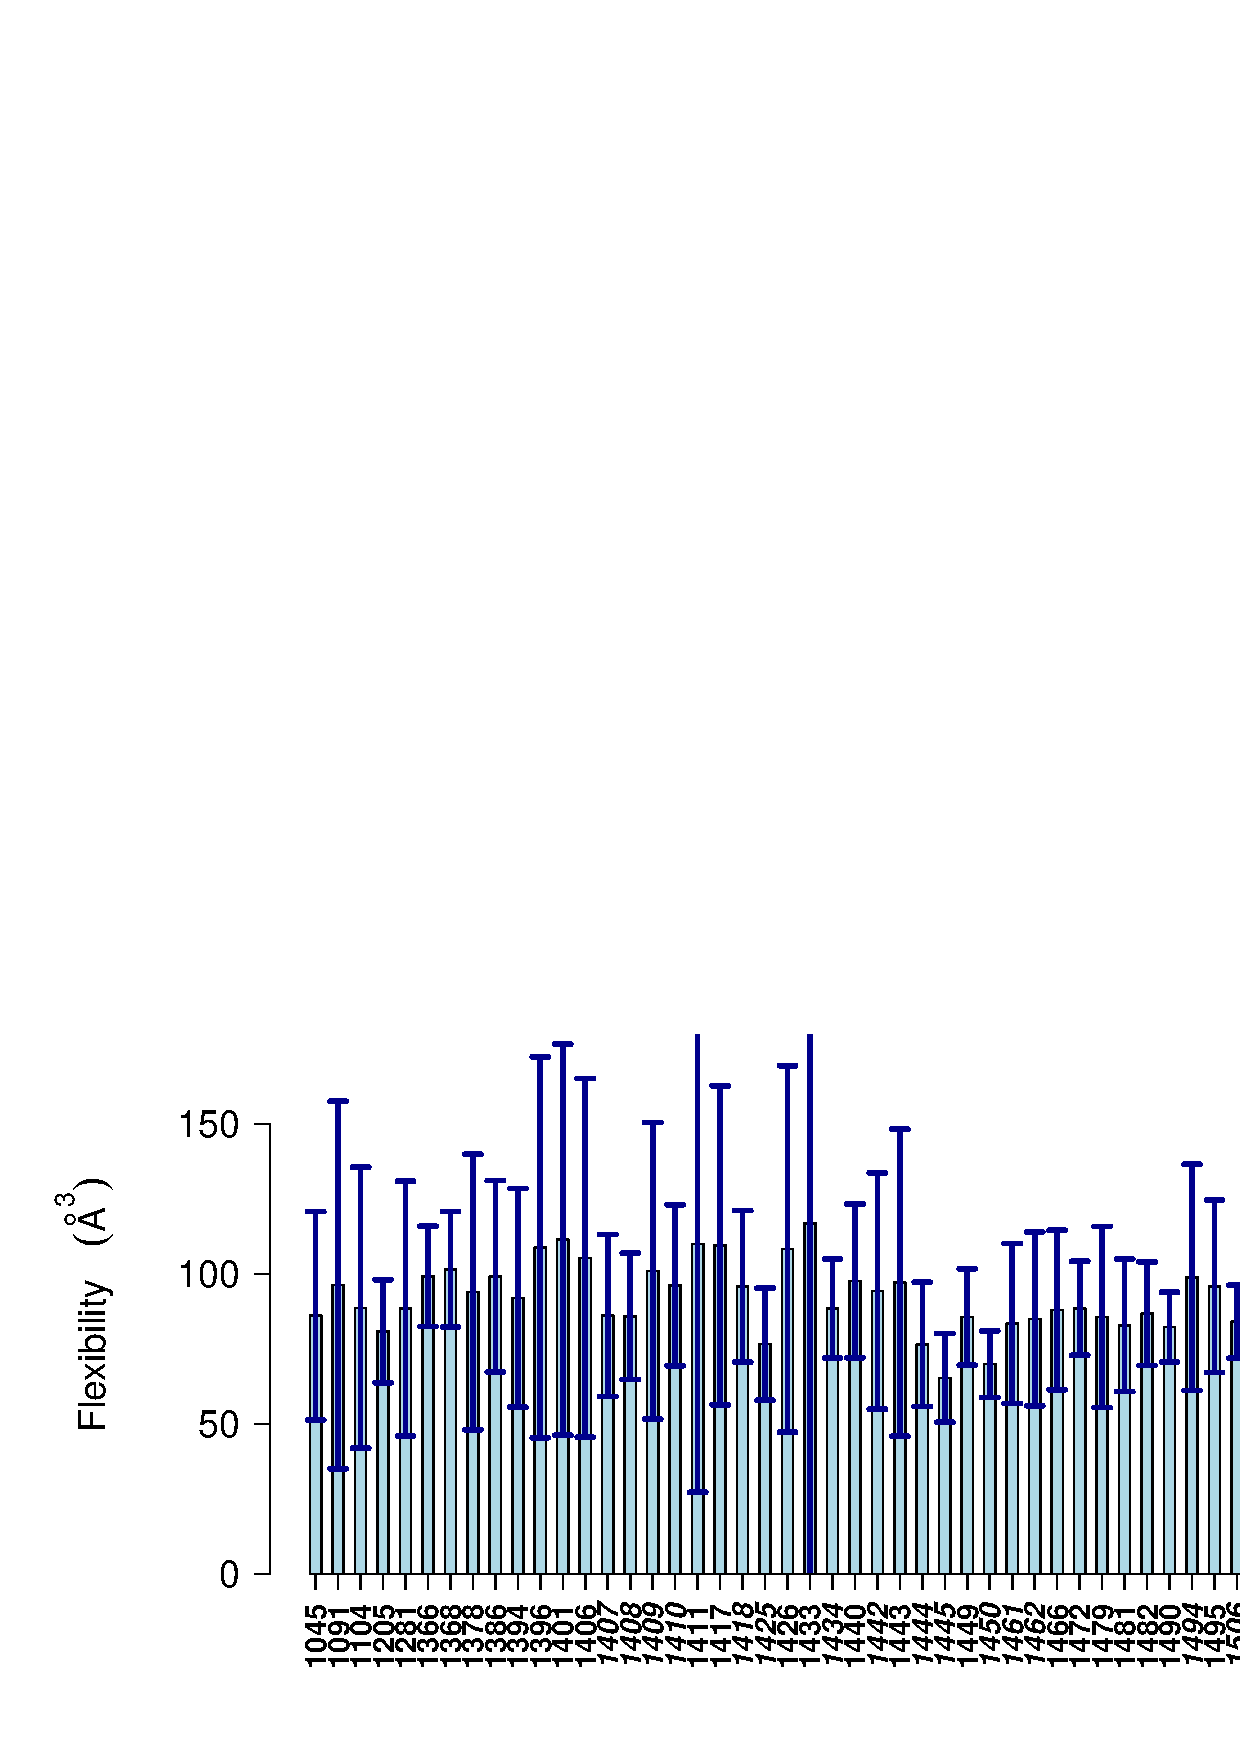
\includegraphics[width=  1 \textwidth]{std-vol}
%	\end{subfigure}
	\caption{The preferred volumes of \numberofreceptors receptors $v_n$ (top). 
		and their flexibilities $\sigma_n$ (down). 
		The error bars are calculated using Jack-Knife method. 
		Some receptors like Or59b, Or67a and  Or85a prefer smaller molecules, 
		but some others like Or19a,  Or1a and  Or49a prefer larger molecules.
		Some receptors like Or46a,  Or22b and Or30a are volume  selective, 
		but some others like Or19a,  Or67b and  Or22a respond to broader range of molecular volumes.
		}
		\label{fig:preferred_volume}
		\label{fig:volume_flexibility}
\end{figure}
 

\end{document}
